\newcommand{\sfill}{white}
\newcommand{\Afill}{white}
\newcommand{\Bfill}{white}
\newcommand{\Cfill}{white}
\newcommand{\Dfill}{white}
\newcommand{\Efill}{white}
\newcommand{\Ffill}{white}
\newcommand{\Gfill}{white}

\begin{tabular}{ccc}

Graph & Queue & Adjazenzliste \\
\gdef\sfill{red}
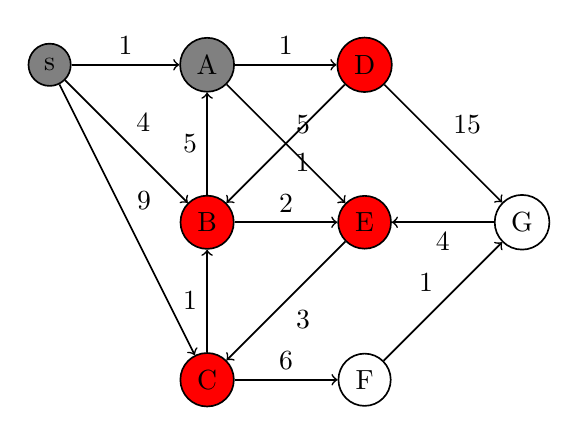
\begin{tikzpicture}[->, semithick,auto, node distance=2cm]


\node[draw, circle, fill=\sfill] (s) at (0,0) {s};
\node[draw, circle, fill=\Afill] (A) [right of=s] {A};
\node[draw, circle, fill=\Bfill] (B) [below of=A] {B};
\node[draw, circle, fill=\Cfill] (C) [below of=B] {C};
\node[draw, circle, fill=\Dfill] (D) [right of=A] {D};
\node[draw, circle, fill=\Efill] (E) [below of=D] {E};
\node[draw, circle, fill=\Ffill] (F) [below of=E] {F};
\node[draw, circle, fill=\Gfill] (G) [right of=E] {G};

\path 	(s) 	edge node {1} (A)
		edge node {4} (B)
		edge node {9} (C)
	(A) 	edge node {1} (D)
		edge node {5} (E)
	(B) 	edge node {5} (A)
		edge node {2} (E)
	(C) 	edge node {1} (B)
		edge node {6} (F)
	(D) 	edge node {1} (B)
		edge node {15} (G)
	(E) 	edge node {3} (C)
	(F) 	edge node {1} (G)
	(G) 	edge node {4} (E)
	;

\end{tikzpicture}

 &
s &
 \\
\gdef\sfill{green}
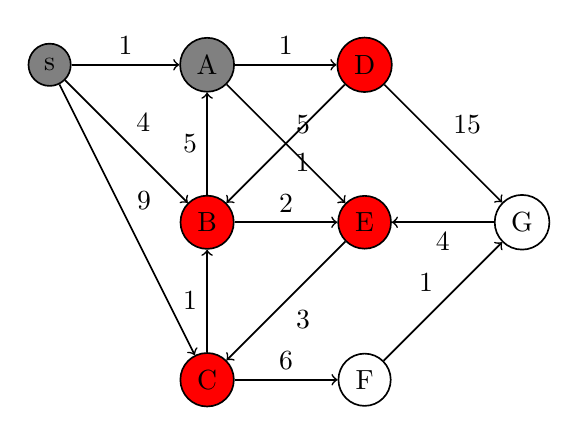
\begin{tikzpicture}[->, semithick,auto, node distance=2cm]


\node[draw, circle, fill=\sfill] (s) at (0,0) {s};
\node[draw, circle, fill=\Afill] (A) [right of=s] {A};
\node[draw, circle, fill=\Bfill] (B) [below of=A] {B};
\node[draw, circle, fill=\Cfill] (C) [below of=B] {C};
\node[draw, circle, fill=\Dfill] (D) [right of=A] {D};
\node[draw, circle, fill=\Efill] (E) [below of=D] {E};
\node[draw, circle, fill=\Ffill] (F) [below of=E] {F};
\node[draw, circle, fill=\Gfill] (G) [right of=E] {G};

\path 	(s) 	edge node {1} (A)
		edge node {4} (B)
		edge node {9} (C)
	(A) 	edge node {1} (D)
		edge node {5} (E)
	(B) 	edge node {5} (A)
		edge node {2} (E)
	(C) 	edge node {1} (B)
		edge node {6} (F)
	(D) 	edge node {1} (B)
		edge node {15} (G)
	(E) 	edge node {3} (C)
	(F) 	edge node {1} (G)
	(G) 	edge node {4} (E)
	;

\end{tikzpicture}

 &
&
 \\
\gdef\Afill{red}
\gdef\Bfill{red}
\gdef\Cfill{red}

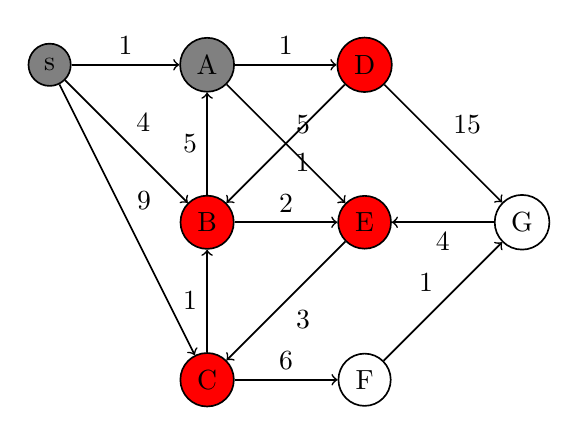
\begin{tikzpicture}[->, semithick,auto, node distance=2cm]


\node[draw, circle, fill=\sfill] (s) at (0,0) {s};
\node[draw, circle, fill=\Afill] (A) [right of=s] {A};
\node[draw, circle, fill=\Bfill] (B) [below of=A] {B};
\node[draw, circle, fill=\Cfill] (C) [below of=B] {C};
\node[draw, circle, fill=\Dfill] (D) [right of=A] {D};
\node[draw, circle, fill=\Efill] (E) [below of=D] {E};
\node[draw, circle, fill=\Ffill] (F) [below of=E] {F};
\node[draw, circle, fill=\Gfill] (G) [right of=E] {G};

\path 	(s) 	edge node {1} (A)
		edge node {4} (B)
		edge node {9} (C)
	(A) 	edge node {1} (D)
		edge node {5} (E)
	(B) 	edge node {5} (A)
		edge node {2} (E)
	(C) 	edge node {1} (B)
		edge node {6} (F)
	(D) 	edge node {1} (B)
		edge node {15} (G)
	(E) 	edge node {3} (C)
	(F) 	edge node {1} (G)
	(G) 	edge node {4} (E)
	;

\end{tikzpicture}

 &

A, B, C&
 \\

\gdef\sfill{gray}
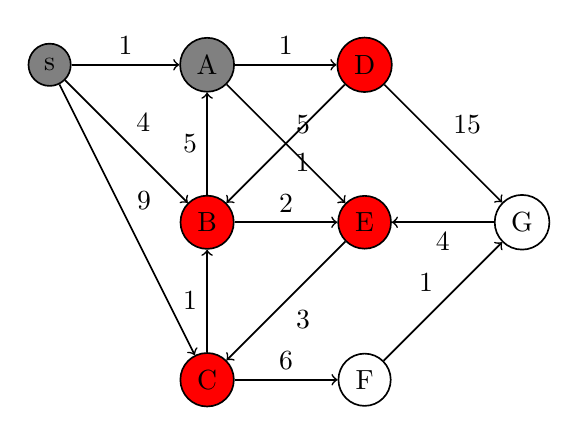
\begin{tikzpicture}[->, semithick,auto, node distance=2cm]


\node[draw, circle, fill=\sfill] (s) at (0,0) {s};
\node[draw, circle, fill=\Afill] (A) [right of=s] {A};
\node[draw, circle, fill=\Bfill] (B) [below of=A] {B};
\node[draw, circle, fill=\Cfill] (C) [below of=B] {C};
\node[draw, circle, fill=\Dfill] (D) [right of=A] {D};
\node[draw, circle, fill=\Efill] (E) [below of=D] {E};
\node[draw, circle, fill=\Ffill] (F) [below of=E] {F};
\node[draw, circle, fill=\Gfill] (G) [right of=E] {G};

\path 	(s) 	edge node {1} (A)
		edge node {4} (B)
		edge node {9} (C)
	(A) 	edge node {1} (D)
		edge node {5} (E)
	(B) 	edge node {5} (A)
		edge node {2} (E)
	(C) 	edge node {1} (B)
		edge node {6} (F)
	(D) 	edge node {1} (B)
		edge node {15} (G)
	(E) 	edge node {3} (C)
	(F) 	edge node {1} (G)
	(G) 	edge node {4} (E)
	;

\end{tikzpicture}

 &
A, B, C&
s \\

\gdef\Afill{green}
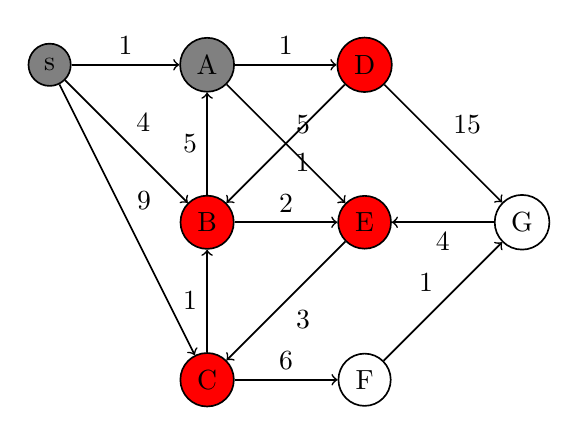
\begin{tikzpicture}[->, semithick,auto, node distance=2cm]


\node[draw, circle, fill=\sfill] (s) at (0,0) {s};
\node[draw, circle, fill=\Afill] (A) [right of=s] {A};
\node[draw, circle, fill=\Bfill] (B) [below of=A] {B};
\node[draw, circle, fill=\Cfill] (C) [below of=B] {C};
\node[draw, circle, fill=\Dfill] (D) [right of=A] {D};
\node[draw, circle, fill=\Efill] (E) [below of=D] {E};
\node[draw, circle, fill=\Ffill] (F) [below of=E] {F};
\node[draw, circle, fill=\Gfill] (G) [right of=E] {G};

\path 	(s) 	edge node {1} (A)
		edge node {4} (B)
		edge node {9} (C)
	(A) 	edge node {1} (D)
		edge node {5} (E)
	(B) 	edge node {5} (A)
		edge node {2} (E)
	(C) 	edge node {1} (B)
		edge node {6} (F)
	(D) 	edge node {1} (B)
		edge node {15} (G)
	(E) 	edge node {3} (C)
	(F) 	edge node {1} (G)
	(G) 	edge node {4} (E)
	;

\end{tikzpicture}

 &
B, C&
s \\

\gdef\Dfill{red}
\gdef\Efill{red}
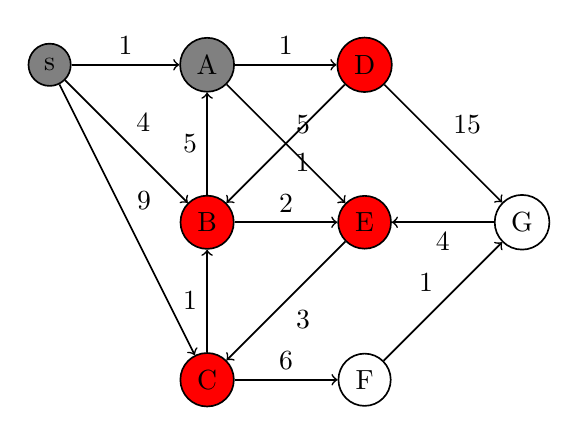
\begin{tikzpicture}[->, semithick,auto, node distance=2cm]


\node[draw, circle, fill=\sfill] (s) at (0,0) {s};
\node[draw, circle, fill=\Afill] (A) [right of=s] {A};
\node[draw, circle, fill=\Bfill] (B) [below of=A] {B};
\node[draw, circle, fill=\Cfill] (C) [below of=B] {C};
\node[draw, circle, fill=\Dfill] (D) [right of=A] {D};
\node[draw, circle, fill=\Efill] (E) [below of=D] {E};
\node[draw, circle, fill=\Ffill] (F) [below of=E] {F};
\node[draw, circle, fill=\Gfill] (G) [right of=E] {G};

\path 	(s) 	edge node {1} (A)
		edge node {4} (B)
		edge node {9} (C)
	(A) 	edge node {1} (D)
		edge node {5} (E)
	(B) 	edge node {5} (A)
		edge node {2} (E)
	(C) 	edge node {1} (B)
		edge node {6} (F)
	(D) 	edge node {1} (B)
		edge node {15} (G)
	(E) 	edge node {3} (C)
	(F) 	edge node {1} (G)
	(G) 	edge node {4} (E)
	;

\end{tikzpicture}

 &
B, C, D, E &
s \\

\gdef\Afill{gray}
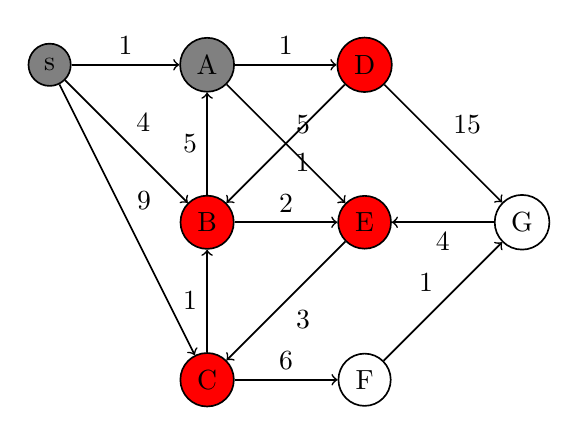
\begin{tikzpicture}[->, semithick,auto, node distance=2cm]


\node[draw, circle, fill=\sfill] (s) at (0,0) {s};
\node[draw, circle, fill=\Afill] (A) [right of=s] {A};
\node[draw, circle, fill=\Bfill] (B) [below of=A] {B};
\node[draw, circle, fill=\Cfill] (C) [below of=B] {C};
\node[draw, circle, fill=\Dfill] (D) [right of=A] {D};
\node[draw, circle, fill=\Efill] (E) [below of=D] {E};
\node[draw, circle, fill=\Ffill] (F) [below of=E] {F};
\node[draw, circle, fill=\Gfill] (G) [right of=E] {G};

\path 	(s) 	edge node {1} (A)
		edge node {4} (B)
		edge node {9} (C)
	(A) 	edge node {1} (D)
		edge node {5} (E)
	(B) 	edge node {5} (A)
		edge node {2} (E)
	(C) 	edge node {1} (B)
		edge node {6} (F)
	(D) 	edge node {1} (B)
		edge node {15} (G)
	(E) 	edge node {3} (C)
	(F) 	edge node {1} (G)
	(G) 	edge node {4} (E)
	;

\end{tikzpicture}

 &
B, C, D, E &
s, A \\

\end{tabular}

